\documentclass[a4paper,11pt]{article}
\usepackage[utf8]{inputenc}
\usepackage{algorithmic}
\usepackage{algorithm}
\usepackage{pst-plot}
\usepackage{graphicx}
\usepackage{endnotes}
\usepackage{graphics}
\usepackage{floatflt}
\usepackage{wrapfig}
	\usepackage{amsfonts}
\usepackage{amsmath}
\usepackage{verbatim}
\usepackage{hyperref}
\usepackage{multirow}
\usepackage{pdflscape}
\usepackage{changepage}
\usepackage{environ}
\usepackage{changepage}
\usepackage{caption}
\usepackage{marginnote}
\reversemarginpar

\usepackage{hyperref}
\hypersetup{pdfborder={0 0 0 0}}

% Matlab listing hightlight
\usepackage[T1]{fontenc}
\usepackage[numbered, framed]{matlab-prettifier}
\let\ph\mlplaceholder
\lstMakeShortInline"
\lstset{
  style              = Matlab-editor,
  basicstyle         = \mlttfamily,
  escapechar         = ",
  mlshowsectionrules = true,
}
\DeclareCaptionFormat{listing}{\par\vskip1pt#1#2#3}
\captionsetup[lstlisting]{format=listing,singlelinecheck=false, margin=0pt, font={sf}, labelsep=space, labelfont=bf}

% Page margins and sizes
\pdfpagewidth 210mm
\pdfpageheight 297mm 
\setlength\topmargin{0mm}
\setlength\headheight{0mm}
\setlength\headsep{0mm}
\setlength\textheight{250mm}	
\setlength\textwidth{159.2mm}
\setlength\oddsidemargin{0mm}
\setlength\evensidemargin{0mm}
\setlength\parindent{0mm}
\setlength\parskip{0mm}

% New environments and commands
\NewEnviron{exercise}[3]{\marginnote{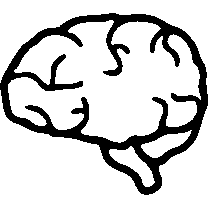
\includegraphics[width=1cm]{brainicon.pdf}\phantom{xx}}[1.2cm]\medskip\paragraph{Exercise #1: #2}\ \\\BODY\ \ \\\phantom{x}\hfill\textbf{\textsc{(#3pt)}}\medskip}
\newcommand{\question}[2]{\setlength\parindent{0mm}\ \\$\mathbf{Q_{#1}:}$ #2\ \\}


% Title
\author{\large{Aqeel Labash, Daniel Majoral, Raul Vicente}}
\title{\huge{Introduction to Computational Neuroscience}\\\LARGE{Practice I: Structure of the Brain}}

\begin{document}
\maketitle

As you might have heard before, structure of the brain is extremely complex. There are lots of neurons next to each other, tangled with each other, forming one, almost gap-less mass. In pursuit of understanding any complex system, one thing you try to learn is its structure. Once you see the structure, you get insights about the purpose of the system. Same, hopefully, stands for our brain. Brain structure consist of neurons, their somas (cell bodies), \emph{dendrites} (input channels), \emph{axons} (output channels) and \emph{synapses} (connection points). 


%
% Exercise: questions about the structure
%
\begin{exercise}{1}{Questionnaire}{2}
\question{1-2}{Does size matter? What is the i) mass and ii) number of neurons in the the brains of the following animals: human, African elephant, horse, giraffe and ant?}
\question{3}{How many synapses are there in the human brain?}
%\question{3}{What is the main objective of the Human Brain Project?}
\question{4}{Compare the bottom-up (biologists) and top-down (engineers, computer scientist) approaches to studying the brain.}
\question{5}{Scientific study of the brain has many branches. Describe in a few examples what are the following fields studying: i)Developmental Neuroscience ii)Clinical Neuroscience iii)Computational neuroscience.}
\question{6}{Why did Golgi think the brain is not comprised of individual cells?}
\question{7}{Why did the nervous system evolve (what is the evolutionary advantage it provides)?}
\question{8}{Name 3 tasks at which computer is much better than human brain and 3 tasks where human brain outperforms any existing computer.}
\question{9}{Describe the main function of the three main compartments of a neuron: soma, dendrite, axon.}
\question{10}{Name two types of glial cells and their functions?}
\question{11}{What is gray matter and white matter?}
\question{12}{The Cerebrum is folded and convoluted to increase the surface area. If you would unfold it, how big would it be (surface area)?}
\question{13}{What types of sensors are are there in the skin?}
\question{14}{If you were to flick a whale's tail, how long it will take for the signal to reach the whale's brain and some response to come back? How long would it take if there was no myelin around the axons? }
\question{15}{What is a neurotransmitter?}
\question{16}{Describe the sequence of actions (ion channels opening and closing) during the generation of an action potential?}
\end{exercise}

%
% Exercise: body and brain masses
%
\begin{exercise}{2}{Body mass vs. brain mass}{1}
In the course of evolution as organisms developed additional organs and functions the system responsible for controlling these functions had to increase as well. In this exercise we will check if it is true that larger animals have larger brain. In the \texttt{data} folder you will find data file \texttt{bodybrain.csv}. It has two columns: the first one is the mass of the animal in kilograms, the second is the mass of its brain in grams.
\begin{enumerate}
	\item Load the data into Matlab/Octave
	\item Create a scatter plot where body mass is on X axis and brain mass on the Y axis (label the axes accordingly)
	\item As you will see the picture is not very interesting, but try plotting in a logarithmic scale (use \texttt{log} function)
	\item What is the relation between the two masses?
\end{enumerate}
\end{exercise}


%
% Exercise: Types of neurons
%
\begin{exercise}{3}{Types of neurons}{1.5}
There are lots of different types of neurons in our nervous system. They have different size, structure and function. Let us have a look at some of them:\\
\ \\
\begin{tabular}{p{3.7cm} p{3.7cm} p{3.7cm} p{3.7cm}}
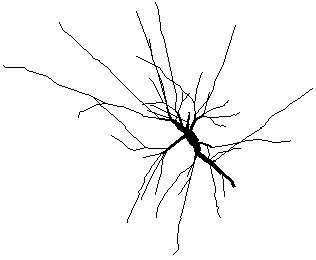
\includegraphics[width=0.25\textwidth]{pyramidal2.png} &
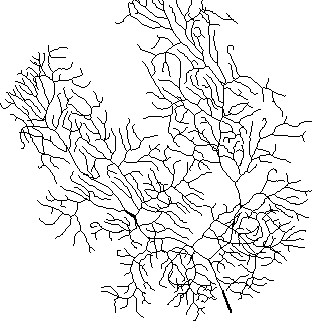
\includegraphics[width=0.25\textwidth]{purkinje.png} &
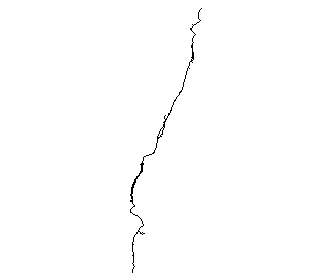
\includegraphics[height=0.25\textwidth]{spindle.png} &
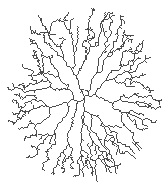
\includegraphics[width=0.25\textwidth]{amacrine.png}\\

\begin{center}\textbf{Pyramidal cell in layer 2 or 3}\end{center}&
\begin{center}\textbf{Purkinje cell}\end{center}&
\begin{center}\textbf{Spindle neuron}\end{center}&
\begin{center}\textbf{Amacrine cell}\end{center} \\
\end{tabular}
\begin{tabular}{p{3.7cm} p{3.7cm} p{3.7cm} p{3.7cm}}
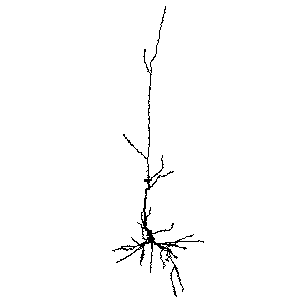
\includegraphics[width=0.25\textwidth]{pyramidal5.png} &
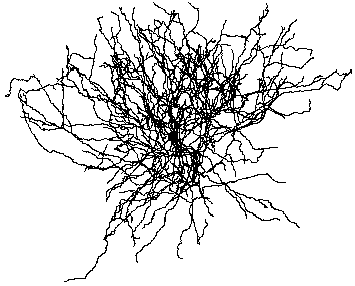
\includegraphics[width=0.25\textwidth]{bascet.png} &
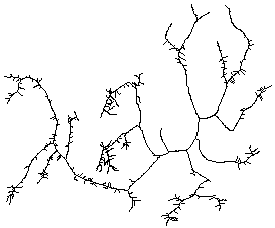
\includegraphics[height=0.25\textwidth]{sensory.png} &
 \\

\begin{center}\textbf{Pyramidal cell in layer 5}\end{center}&
\begin{center}\textbf{Basket cell}\end{center}&
\begin{center}\textbf{Sensory neuron}\end{center}&
\begin{center}\textbf{}\end{center} \\
\end{tabular}


In the \texttt{data} folder of this assignment you will find three \texttt{.swc} files. Each file describes reconstructed structure of a neuron. A neuron can be characterized by different parameters, such as size, bifurcations (branching points), size of soma, etc. In general the task of identifying the type of a neuron is quite hard\footnote{M. Bota, L. W. Swanson, \textbf{The neuron classification problem}, 2007, 
\url{http://www.sciencedirect.com/science/article/pii/S0165017307000768}}. \\
Nevertheless, in some cases, different types of neurons have distinguishable shapes. This is what we will try to use in this exercise. Your task is to plot neurons from the data files and guess which of the above-mentioned types each of them belongs to.
\begin{enumerate}
	\item Have a look inside an \texttt{.swc} file. Each line describes small piece of the neuron (\emph{compartment}), the values in the columns are: 
	\begin{enumerate}
		\item ID of the compartment
		\item Type of the compartment:
		\begin{enumerate}
			\item[0] -- undefined
			\item[1] -- soma
			\item[2] -- axon
			\item[3] -- basal dendrite
			\item[4] -- apical dendrite
		\end{enumerate}
		\item X coordinate (in $\mu$m)
		\item Y coordinate
		\item Z coordinate	
		\item Radius of the compartment
		\item ID of parent compartment (-1 for root compartment)
	\end{enumerate}
	\item Import the 3 coordinates of all compartments into your program (you can use any programming language/environment)
	\item Plot the data in 3D (for example using \texttt{scatter3} in \texttt{Matlab})
	\item Look at the resulting 3D image an try to guess type of the neuron
	\item (optional) If you are not sure about the neuron type based on the scatter plot, feel free to draw lines between connected compartments (each compartment is connected to its parent compartment, so you need to draw a line segment for each parent-child pair).
\end{enumerate}
\ \\
In your report please report the probable type of the neuron for each of the files, include visualizations (pictures from different angles) and the code to reproduce them. You can use \texttt{Matlab/Octave}, \texttt{R}, \texttt{Python} or any other programming language (Only for this home work).
\end{exercise}

%
% Exercise: brain lesions
%
\begin{exercise}{4}{Brain lesions}{1}
Brain \emph{lesions} are abnormalities in the structure of the brain, usually due to damage after accidents, strokes etc. Some lesions lead to interesting effects, that give us information about the functional role of the damaged region - if after damage to some region you cannot see any more, then probably that area was crucial for vision. \\
Read about brain lesions and their possible consequences. Google up one lesion, which has surprising or informative (about function) consequences, and:
\begin{itemize}
\itemsep 0em
	\item describe the nature of the lesion
	\item find a picture of the structure that is damaged, altered or disturbed
	\item tell about its characteristics, e.g. is it temporal or permanent
	\item describe the consequences
	\item speculate on how the effect is related to the functional role of that region
\end{itemize}
(for motivated people) Alternatively, you can describe an interesting transcranial magnetic stimulation (TMS) study.
\end{exercise}


\ \\
\ \\
\ \\
\ \\
\ \\
Please submit a \texttt{pdf} report with answers to the questions and comments about your solutions. Include figures, explanations and essential pieces of code. Do not include the code itself as a separate file, your report should give good understanding of what you have done. Please mark how long it took to complete this set of exercises, including time spent in the practical session itself. Upload the \texttt{pdf} to the practice session page on the course website. If worked with someone else (discussed) mention him at the end of your report. Any answer copying will yield a zero for the whole practice, for all students implied.
\end{document}